%% ---------------------------------------------------------------------------
%% Two-page IEEE conference paper — architecture and operation of the system.
%% Written in plain language for a non-specialist reader.
%% Built with the official IEEEtran class (v1.8b), bundled in this directory.
%%
%% Compile:  pdflatex paper.tex   (run twice, so the figure reference resolves)
%% ---------------------------------------------------------------------------
\documentclass[conference]{IEEEtran}

\usepackage[T1]{fontenc}
\usepackage[utf8]{inputenc}
\usepackage{tikz}
\usetikzlibrary{arrows.meta,positioning,calc}
\usepackage{booktabs}
\usepackage{graphicx}
\usepackage{microtype}
\usepackage{xcolor}

%% palet biru pastel untuk diagram, dan biru tua untuk tautan
\definecolor{linkblue}{HTML}{1F4E79}
\definecolor{inkblue}{HTML}{1F4E79}
\definecolor{pastelblue}{HTML}{E3EEF9}
\definecolor{pastelbluedeep}{HTML}{C2D9EF}

\usepackage[colorlinks=true,allcolors=linkblue,breaklinks=true]{hyperref}
\usepackage{url}

\hyphenation{ac-cre-di-ta-tion re-triev-al doc-u-ment}

\begin{document}

\title{Grounded Local AI for University Accreditation}

\author{\IEEEauthorblockN{Alfa Yohannis}
\IEEEauthorblockA{\textit{Faculty of Science and Technology} \\
\textit{Pradita University}, Tangerang, Indonesia \\
alfa.ryano@pradita.ac.id}}

\maketitle

\begin{abstract}
Preparing a university accreditation submission means answering hundreds of
detailed questions, and the evidence for each is buried somewhere in a shared
folder of thousands of files. This paper describes a working system that lets
staff ask a question in everyday Indonesian and receive an answer in seconds, in
which every statement carries a numbered citation pointing to the exact file and
page it came from. It is built on retrieval-augmented generation: the
institution's own documents are searched first, and the language model may write
only from what was found. We explain the architecture in plain terms and the
design choices that make the answers checkable---source files are never
modified, and the whole system runs on one office workstation, so confidential
material need not leave the building.
\end{abstract}

\begin{IEEEkeywords}
retrieval-augmented generation, document question answering, accreditation,
hybrid retrieval, large language models, higher education
\end{IEEEkeywords}

\section{The Problem}

An accreditation submission is an exercise in evidence. For every claim a study
programme makes---about its curriculum, its lecturers, its graduates, its
research---an assessor may ask where the proof is. The proof exists: in a decree
issued three years ago, in row~47 of a spreadsheet, on page~12 of a curriculum
document. It is simply spread across thousands of files accumulated over years
in a shared drive that several colleagues edit at once.

The consequence is familiar: a single question can cost half an hour of opening
files one by one, and under deadline pressure the tempting shortcut is to answer
from memory---which is how an unsupported claim reaches an assessor. A
general-purpose chatbot does not help, having never seen these documents yet
still producing a fluent answer that cites nothing. What is needed is a system
that answers \emph{only} from the institution's own files, and shows its
working.

\section{What the User Sees}

The system is a web page that opens in any browser on the office network,
including a phone, offering a single box for a question in Indonesian. Seconds
later an answer appears in ordinary prose, a small numbered marker beside each
statement, and beside it an evidence panel: one card per marker giving the
document's name, the page or sheet the passage came from, and the passage
itself. Clicking a card opens the original file. The user is therefore never
asked to trust the system---every sentence can be checked in one click.

Asked whether the programme teaches machine learning, for instance, the system
replies that the curriculum lists a \emph{Machine Learning and Deep Learning}
course, and attaches the curriculum spreadsheet and the sheet its course table
sits on, so the reader can open it and see the row.

\section{Architecture}

Fig.~\ref{fig:arch} shows the system twice over: panel~(a) follows a question
from the shared folder to a cited answer, panel~(b) shows the same system as
components. The backend is Python; the browser interface is plain JavaScript,
with no framework and no build step.

\begin{figure*}[t]
\centering
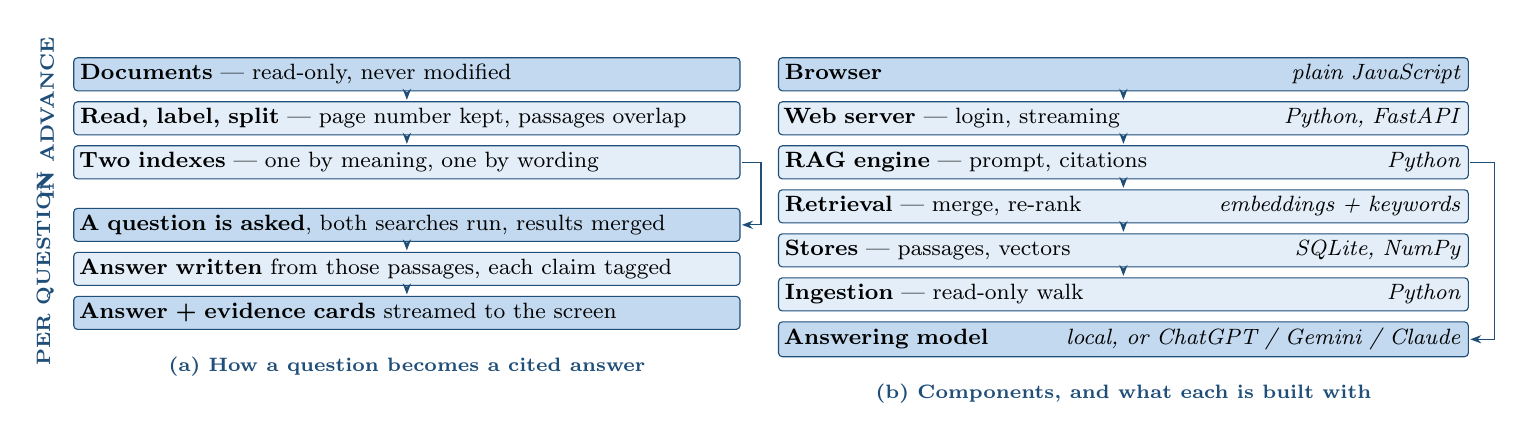
\begin{tikzpicture}[
  node distance=1.25mm,
  box/.style={draw=inkblue, line width=0.4pt, fill=pastelblue,
              rounded corners=1.4pt, align=left, font=\fontsize{8}{9.6}\selectfont,
              inner sep=2.3pt, text width=83mm, minimum height=4.2mm},
  cmp/.style={draw=inkblue, line width=0.4pt, fill=pastelblue,
              rounded corners=1.4pt, align=left, font=\fontsize{8}{9.6}\selectfont,
              inner sep=2.3pt, text width=86mm, minimum height=4.2mm},
  ar/.style={-{Stealth[length=1.4mm]}, draw=inkblue, line width=0.4pt,
             shorten >=0.5pt, shorten <=0.5pt},
  lbl/.style={font=\scriptsize\bfseries, text=inkblue}
]

%% ---------------- panel (a): what happens to a question ----------------
\begin{scope}
\node[box, fill=pastelbluedeep] (src)
  {\textbf{Documents} --- read-only, never modified};
\node[box, below=of src] (prep)
  {\textbf{Read, label, split} --- page number kept, passages overlap};
\node[box, below=of prep] (index)
  {\textbf{Two indexes} --- one by meaning, one by wording};

\node[box, below=3.6mm of index, fill=pastelbluedeep] (search)
  {\textbf{A question is asked}, both searches run, results merged};
\node[box, below=of search] (ans)
  {\textbf{Answer written} from those passages, each claim tagged};
\node[box, below=of ans, fill=pastelbluedeep] (out)
  {\textbf{Answer + evidence cards} streamed to the screen};

\foreach \a/\b in {src/prep, prep/index, search/ans, ans/out}
  \draw[ar] (\a) -- (\b);
\draw[ar] (index.east) -- ++(2.6mm,0) |- (search.east);

\node[lbl, rotate=90, anchor=south]
  at ([xshift=-1.2mm]$(src.west)!0.5!(index.west)$) {IN ADVANCE};
\node[lbl, rotate=90, anchor=south]
  at ([xshift=-1.2mm]$(search.west)!0.5!(out.west)$) {PER QUESTION};
\node[lbl, below=2.2mm of out] {(a) How a question becomes a cited answer};
\end{scope}

%% ---------------- panel (b): components and technology ----------------
\begin{scope}[xshift=91mm]
\node[cmp, fill=pastelbluedeep] (ui)
  {\textbf{Browser} \hfill \textit{plain JavaScript}};
\node[cmp, below=of ui] (srv)
  {\textbf{Web server} --- login, streaming \hfill \textit{Python, FastAPI}};
\node[cmp, below=of srv] (rag)
  {\textbf{RAG engine} --- prompt, citations \hfill \textit{Python}};
\node[cmp, below=of rag] (ret)
  {\textbf{Retrieval} --- merge, re-rank \hfill \textit{embeddings + keywords}};
\node[cmp, below=of ret] (sto)
  {\textbf{Stores} --- passages, vectors \hfill \textit{SQLite, NumPy}};
\node[cmp, below=of sto] (ing)
  {\textbf{Ingestion} --- read-only walk \hfill \textit{Python}};
\node[cmp, below=of ing, fill=pastelbluedeep] (llm)
  {\textbf{Answering model} \hfill \textit{local, or ChatGPT / Gemini / Claude}};

\foreach \a/\b in {ui/srv, srv/rag, rag/ret, ret/sto, sto/ing}
  \draw[ar] (\a) -- (\b);
\draw[ar] (rag.east) -- ++(3.2mm,0) |- (llm.east);
\node[lbl, below=2.2mm of llm] {(b) Components, and what each is built with};
\end{scope}

\end{tikzpicture}
\caption{Architecture of the system. In panel~(a) the upper half runs whenever
documents change and the lower half runs in seconds each time somebody asks.
Arrows point in the direction work flows; note in panel~(b) that the answering
model is reached only through the RAG engine, and never touches the document
store itself.}
\label{fig:arch}
\end{figure*}

\subsection{Reading the documents}

The system walks the shared drive and opens every file it understands---PDF,
Word, Excel, PowerPoint, web pages, plain text, and scanned images through
optical character recognition---and pulls the words out. Crucially, it remembers
\emph{where} each piece of text was: page~12, sheet ``Dosen'', slide~4. That
bookkeeping is what makes a citation possible later.

Evidence on public websites---the ministry's database, research profiles, staff
pages---is fetched once, saved as a dated copy, and thereafter indexed like any
other document. Long documents are split into passages of a few hundred words that overlap
slightly at the edges, so a fact straddling a boundary is never cut in two.
Re-running the process re-reads only files that actually changed, detected from
each file's size and modification time, so a daily update takes seconds rather
than the tens of minutes a full pass costs.

\subsection{Two kinds of search}

Every passage is filed in two separate indexes, because the two ways of searching
fail in different places.

\textbf{Search by meaning} converts each passage into a list of numbers---an
embedding~\cite{bge}---capturing what the text is about. The question is
converted the same way, and the closest passages are returned. This understands
that ``lecturer teaching load'' and the abbreviation ``EWMP'' mean the same
thing though they share no words, but it is unreliable with exact identifiers.

\textbf{Search by exact wording} is ordinary keyword search~\cite{bm25}. It
finds a decree number such as \texttt{SK-045/XYZ/VI/2025} precisely, and is
blind to paraphrase.

Accreditation documents are full of both: narrative argument on one page,
decree and registration numbers on the next. Dropping either method would
quietly make a whole class of questions unanswerable.

The two result lists cannot simply be added, because their scores are on
different scales. The system merges them by \emph{position} instead: a passage
ranked highly by both methods is promoted above one only a single method
favours. This is reciprocal rank fusion~\cite{rrf}, and it needs no retuning when
the collection changes. The two dozen survivors are then read once more, in
full, against the question by a second, slower model that scores
question--passage pairs directly, and only the best handful is carried forward.

\subsection{Writing the answer}

Only those final passages are handed to a language model, with an instruction to
answer from them alone and to tag each statement with the number of the passage
supporting it. This arrangement---search first, then write only from what was
found---is retrieval-augmented generation~\cite{lewis}. The model cannot browse
the web, open files or run commands, and is instructed to say so when the
passages do not contain the answer. The evidence cards reach the browser
\emph{before} the first word of the answer, so the reader can start checking
sources while it is still being written.

\subsection{Choosing the model}

The answering model is interchangeable, and the choice is a privacy decision
more than a technical one. By default an 8-billion-parameter model~\cite{qwen}
runs \emph{locally}, so no document text leaves the building; for harder
questions the operator may select ChatGPT, Gemini or Claude, which synthesise
better but send the retrieved passages outside. The interface states the
trade-off on the selector itself, so the choice is made knowingly.

\section{Design Decisions}

\emph{Source documents are never modified.} The shared drive is the real
evidence archive, edited daily, so the rule is enforced in software: every file
operation passes through a guard that refuses to open a source file for writing,
and the server refuses to start if its own working folder sits inside the
archive. A test verifies that a full indexing pass leaves every file
byte-for-byte identical.

\emph{External evidence is frozen, not fetched.} Public pages change, so the
system cites its dated copy rather than the live page---while still linking to
it---so that an assessor sees the page that was actually quoted.

\emph{Answers survive lost connections.} Answers are produced on the server
independently of the requesting browser, with every event numbered, so a user
whose connection drops resumes exactly where the text left off.

\section{Deployment and Scale}

The system is in use for a Master's programme accreditation submission. The
index covers \textbf{1{,}497 documents}---about 188{,}000 sentences and 3.5
million words. It runs on one desktop---a 20-core Core i7-14700F, 32\,GB of
memory, an RTX 4060 with 8\,GB of video memory---and 7.4\,GB of disk, mostly the
downloaded models. Answers take seconds to under a minute. That single machine serves the whole team,
with a full-privilege account for the administrator and a read-only account for
everyone else.

\section{Conclusion}

The contribution is not a new algorithm but a demonstration: an accreditation
team can have a question-answering assistant whose answers are \emph{checkable
by construction}---built from its own documents, citing them by page, leaving
them untouched, and running on hardware the department already owns. The
approach transfers to any organisation that must justify claims from a large,
messy, authoritative archive.

\begin{thebibliography}{9}
\footnotesize

\bibitem{lewis}
P. Lewis \emph{et al.}, ``Retrieval-augmented generation for knowledge-intensive
NLP tasks,'' in \emph{Proc. NeurIPS}, 2020, pp. 9459--9474. [Online]. Available:
\url{https://arxiv.org/abs/2005.11401}

\bibitem{rrf}
G. V. Cormack, C. L. A. Clarke, and S. Buettcher, ``Reciprocal rank fusion
outperforms Condorcet and individual rank learning methods,'' in \emph{Proc.
32nd ACM SIGIR Conf.}, 2009, pp. 758--759. [Online]. Available:
\url{https://doi.org/10.1145/1571941.1572114}

\bibitem{bge}
J. Chen, S. Xiao, P. Zhang, K. Luo, D. Lian, and Z. Liu, ``M3-Embedding:
Multi-linguality, multi-functionality, multi-granularity text embeddings through
self-knowledge distillation,'' arXiv:2402.03216, 2024. [Online]. Available:
\url{https://arxiv.org/abs/2402.03216}

\bibitem{bm25}
S. Robertson and H. Zaragoza, ``The probabilistic relevance framework: BM25 and
beyond,'' \emph{Found. Trends Inf. Retr.}, vol. 3, no. 4, pp. 333--389, 2009.
[Online]. Available: \url{https://doi.org/10.1561/1500000019}

\bibitem{qwen}
A. Yang \emph{et al.} (Qwen Team), ``Qwen3 technical report,'' arXiv:2505.09388,
2025. [Online]. Available: \url{https://arxiv.org/abs/2505.09388}

\end{thebibliography}

\end{document}
